\documentclass{beamer}
\setbeamertemplate{navigation symbols}{}

\usepackage{beamerthemeshadow}
\usepackage{algorithm}
\usepackage{float}
\usepackage{algpseudocode}
\usepackage{hyperref}
\usepackage{multirow}
\usepackage{array}
\usepackage{booktabs}
\usepackage{makecell}

\begin{document}
\title{Study of near collisions in reduced versions of BLAKE, Gr{\o}stl and Keccak}  
\author{Soham Sadhu}
\institute{Capstone Project Committee \\
Prof. Stanis{\l}aw Raziszowski \\
Prof. Leon Reznik \\
Prof. Xumin Liu}
\date{August 22, 2014} 

\begin{frame}
\titlepage
\end{frame}

%\begin{frame}
%\frametitle{Abstract}
%\begin{itemize}
%\item Cryptographic hash functions are used to create and verify digital signatures.
%\item U.S government standardizes the hash function to be used in all non military government 
%agency through Federal Information and Processing Standards (FIPS) publications for
%Secure Hashing Algorithm (SHA).
%\item In October 2012, Keccak was chosen as the winner of SHA-3 competition amongst 64 candidates, including 
%the finalists BLAKE and Gr{\o}stl.
%\item We study near collisions in reduced versions of BLAKE, Gr{\o}stl and Keccak; using hill
%climbing, random selection, simulated annealing and tabu search.
%\end{itemize}
%\end{frame}

\begin{frame}
  \frametitle{Summary}
  \begin{itemize}
    \item Reduced versions of BLAKE, Gr{\o}stl and Keccak, compared on basis of near collisions.
    \item Hill climbing, simulated annealing, tabu search and random selection used to find near 
      collisions.
  \end{itemize}
\end{frame}

\begin{frame}[allowframebreaks]{Outline}
\frametitle{Table of contents}
\tableofcontents
\end{frame} 

\section{Introduction}

\subsection{Hash function}
\begin{frame}
  \frametitle{Hash function}
  A \emph{hash family} is a four-tuple ($\mathcal{X}, \mathcal{Y}, \mathcal{K}, \mathcal{H}$),
  satisfying the following conditions.\footnotemark
  \begin{itemize}
    \item $\mathcal{X}$ is a set of possible messages
    \item $\mathcal{Y}$ is a finite set of hash function output
    \item $\mathcal{K}$, the \emph{keyspace}, is a finite set of possible keys
    \item For each $K \in \mathcal{K}$, there is a hash function $h_{k} \in \mathcal{H}$. Each 
      $h_{k}: \mathcal{X} \to \mathcal{Y}$ 
  \end{itemize}
  \footnotetext[1]{Douglas R. Stinson. Cryptography Theory and Practice, chapter 4. Cryptographic
  Hash Functions. Chapman \& Hall/CRC, Boca Raton, FL 33487-2742, USA, third edition, 2006.}
\end{frame}

\subsection{Property of hash function}
\begin{frame}
  \frametitle{Property of Hash function\footnotemark}
  \begin{enumerate}
  \item {\bf Preimage resistance} \\
  {\bf Given:} A hash function $h : \mathcal{X} \to \mathcal{Y}$ and an element $y \in \mathcal{Y}$. \\
  {\bf Find:} $x \in \mathcal{X}$ such that $h(x) = y$.
  \item {\bf Second preimage} \\
  {\bf Given:} A hash function $h : \mathcal{X} \to \mathcal{Y}$ and an element $x \in \mathcal{X}$. \\
  {\bf Find:} $x' \in \mathcal{X}$ such that $x' \neq x$ and $h(x) = h(x')$.
  \item {\bf Collision resistance} \\
  {\bf Given:} A hash function $h : \mathcal{X} \to \mathcal{Y}$ \\
  {\bf Find:} $x, x' \in \mathcal{X}$ such that $x' \neq x$ and $h(x') = h(x)$. 
  \end{enumerate}
  \footnotetext[2]{Douglas R. Stinson. Cryptography Theory and Practice, chapter 4. Cryptographic
  Hash Functions. Chapman \& Hall/CRC, Boca Raton, FL 33487-2742, USA, third edition, 2006.}
\end{frame}

%\subsection{Security model}
%\begin{frame}
%\frametitle{Security model}
%\begin{itemize}
%\item {\bf Random Oracle} model, proposed by Bellare and Rogaway. Algorithm is secure, modulo the way it creates
%the random outputs.\footnotemark
%\item {\bf Birthday paradox:} In a sample size of $M$, minimum $N$ number of attempts to find, two elements with
%same value is given by equation $N \approx 1.17 \sqrt{M}$. 
%\end{itemize}
%\footnotetext[3]{Gerrit Bleumer. Random oracle model. In HenkC.A. van Tilborg and Sushil Jajodia,
%editors, Encyclopedia of Cryptography and Security, pages 1027–1028. Springer US, 2011.}
%\end{frame}

\subsection{Application}
\begin{frame}
\frametitle{Application of hash functions}
\begin{enumerate}
\item Digital signature
\item Digital forensics \footnotemark
\item Password stored 
\item File integrity
\item Pseudo random string generator
\end{enumerate}
\footnotetext[3]{Richard P. Salgado. Fourth Amendment Search And The Power Of The Hash, volume
119 of 6, pages 38 – 46. Harvard Law Review Forum, 2006.}
\end{frame}

\subsection{Standards and SHA-3 competition}

\begin{frame}
  \frametitle{SHA}
  \begin{enumerate}
    \item SHA-0 proposed by NSA in 1993, later standardized by NIST.
    \item SHA-1 designed by NSA in 1995, digest 160 bits, block size 512 bits \footnotemark.
    \item SHA-2 released by NIST in 2001. Family of hash functions of size 224, 256, 384 and 512 bits.
    \item 
  \end{enumerate}
  \footnotetext[4]{James Joshi. Network Security: Know It All: Know It All. Newnes Know It All. Elsevier Science, 2008.}
\end{frame}

%\begin{frame}
%\frametitle{SHA-0}
%\begin{itemize}
%\item SHA-0 proposed by NSA in 1993, later standardised by NIST. 
%\item In 1995 Florent Chabaud and Antoine Joux, found collisions in SHA-0 with complexity of $2^{61}$.
%\item In 2004, Eli Biham and Chen found near collisions for SHA-0, about 142 out of 160 bits to be equal.
%\item Full collisions were also found, when the number of rounds for the algorithm were reduced from 80 to 62.
%\end{itemize}
%\end{frame}

%\begin{frame}
%\frametitle{SHA-1}
%\begin{itemize}
%\item In 1995, SHA-0 replaced by SHA-1, designed by NSA\footnotemark. SHA-1 had block size of 512 bits, size of 
%160 bits; and additional circular shift operation, to rectify weakness from SHA-0.
%\item In 2005, team from Shandong University found collisions on full version of SHA-1 requiring $2^{69}$ 
%operations\footnotemark.
%\end{itemize}
%\footnotetext[4]{James Joshi. Network Security: Know It All: Know It All. Newnes Know It All. Elsevier Science, 2008.}
%\footnotetext[5]{Bruce Schneier. Sha-1 broken.
%http://www.schneier.com/blog/archives/2005/02/sha1\_broken.html, February 2005.}
%\end{frame}

%\begin{frame}
%\frametitle{SHA-2}
%\begin{itemize}
%\item SHA-2 was designed by NSA, and released in 2001 by NIST. Family of functions of SHA-224, SHA-256, 
%SHA-384, SHA-512.
%\item Computational operations for finding collisions in SHA-256 for 23-step was found to be around 
%$2^{11.5}$, and for 24 step was $2^{28.5}$ respectively.
%\item Computational operations for finding collisions in SHA-512 for 23-step was found to be around 
%$2^{16.5}$, and for 24 step was $2^{32.5}$ respectively\footnotemark.
%\end{itemize}
%\footnotetext[6]{Somitra Kumar Sanadhya and Palash Sarkar. New collision attacks against up to 24-
%step sha-2. In Dipanwita Roy Chowdhury, Vincent Rijmen, and Abhijit Das, editors, INDOCRYPT, volume 5365 
%of Lecture Notes in Computer Science, pages 91–103. Springer, 2008.}
%\end{frame}

%\begin{frame}
%\frametitle{SHA-3}
%\begin{itemize}
%\item NIST announced competition for choosing SHA-3 on November, 2007. Entries accepted till October, 2008.
%\item 51 candidates from 64 submissions, were accepted for first round on December 9, 2008.
%\item Out of 5 finalists, on October 2, 2012; Keccak was announced winner amongst other four finalist, which
%included BLAKE and Gr{\o}stl.
%\item Keccak was chosen for large security margin, flexibility, and efficient hardware implementation.
%\end{itemize}
%\end{frame}

\section{SHA-3}

\subsection{FIPS PUB 202}

\begin{frame}
\frametitle{FIPS PUB 202\footnotemark}
SHA3-224(M) = KECCAK[448](M $\vert \vert$ 01, 224) \\
SHA3-256(M) = KECCAK[512](M $\vert \vert$ 01, 256) \\
SHA3-384(M) = KECCAK[768](M $\vert \vert$ 01, 384) \\
SHA3-512(M) = KECCAK[1024](M $\vert \vert$ 01, 512) \\
SHAKE128(M, d) = KECCAK[256](M $\vert \vert$ 1111, d) \\
SHAKE256(M, d) = KECCAK[512](M $\vert \vert$ 1111, d)
\footnotetext[7]{Information Technology Laboratory, National Institute of Standards and Technology.
DRAFT FIPS PUB 202, SHA-3 Standard: Permutation Based Hash and Extendable-Output Functions. May 2014.}
\end{frame}

\subsection{Keccak}

\begin{frame}
\frametitle{Keccak sponge construction}
\begin{figure}[h]
  \begin{center}
    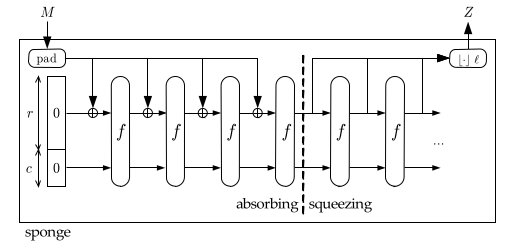
\includegraphics[scale=0.5]{keccakspongeconstruction.jpg}
  \end{center}
  \caption{Sponge construction $Z = Sponge[f, pad, r](M, l)$\footnotemark}
  \label{fig:lab}
\end{figure}
\footnotetext[8]{Guido Bertoni, Joan Daemen, Micha\"{e}l Peeters, and Gilles Van Assche. Cryptographic
sponge functions. http://sponge.noekeon.org/CSF-0.1.pdf, January 2011.}
\end{frame}

\begin{frame}
\frametitle{Keccak state}
\begin{figure}[h]
  \begin{center}
    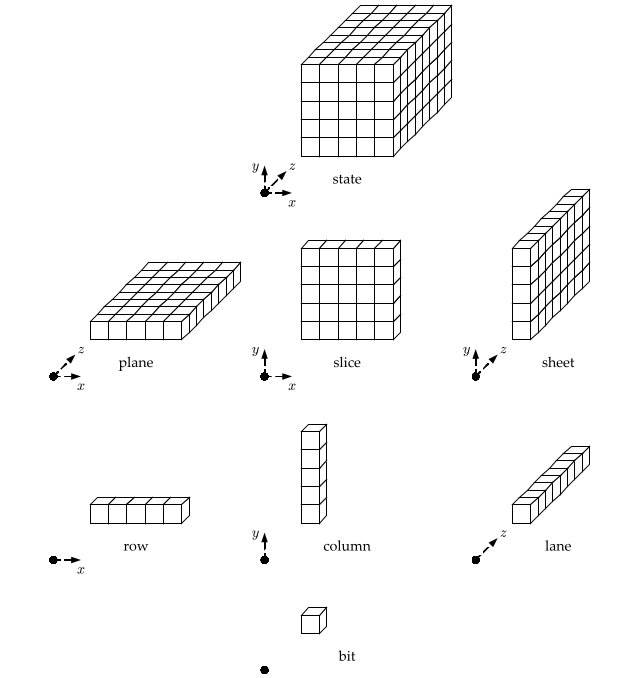
\includegraphics[scale=0.25]{keccakstateterminology.jpg}
  \end{center}
  \caption{Keccak state terminology $Z = Sponge[f, pad, r](M, l)$\footnotemark}
  \label{fig:lab}
\end{figure}
\footnotetext[22]{Guido Bertoni, Joan Daemen, Micha\"{e}l Peeters, and Gilles Van Assche. The keccak 
reference. http://keccak.noekeon.org/Keccak-reference-3.0.pdf, January 2011.}
\end{frame}

\begin{frame}
\frametitle{Padding and permutations}
\begin{itemize}
\item The message is padded with $1 0^{*}1$ to make it multiple of the block length.
\item $R = \iota \circ \chi \circ \pi \circ \rho \circ \theta$
\item The permutation round R is repeated for 12 + 2l times, where l is the lane length. The default
capacity size is 576.
\end{itemize}
\end{frame}

\begin{frame}
\frametitle{Contents of Keccak permutation round}
\begin{align*}
  \theta &: a[x][y][z] & \gets & \thickspace a[x][y][z] + \displaystyle\sum\limits_{y' = 0}^{4} a[x - 1][y'][z] + \displaystyle\sum\limits_{y' = 0}^{4} a[x + 1][y'][z - 1], \\
  \rho &: a[x][y][z] & \gets & \thickspace a[x][y][z - (t + 1)(t + 2) / 2], \\
  & & & \thickspace t \thickspace satisfying \thickspace 0 \leq t < 24 \thickspace and \thickspace
  \begin{pmatrix} 0 & 1 \\ 2 & 3 \end{pmatrix}^{t} \begin{pmatrix} 1 \\ 0 \end{pmatrix} = \begin{pmatrix} x \\ y \end{pmatrix}
  in \thickspace GF(5)^{2 \times 2}, \\
  & & & \thickspace or \thickspace t = -1 \thickspace if \thickspace x = y = 0, \\
  \pi &: a[x][y] & \gets & \thickspace a[x'][y'], \thickspace with \thickspace
  \begin{pmatrix} x \\ y \end{pmatrix} = \begin{pmatrix} 0 & 1 \\ 2 & 3 \end{pmatrix} \begin{pmatrix} x' \\ y'\end{pmatrix}, \\
  \chi &: a[x] & \gets & \thickspace a[x] + (a[x + 1] + 1) \thickspace a[x + 2], \\
  \iota &: a & \gets & \thickspace a + RC[i_{r}].
\end{align*}
\end{frame}

%\begin{frame}
%\frametitle{$\theta$ step}
%\begin{figure}[h]
  %\begin{center}
    %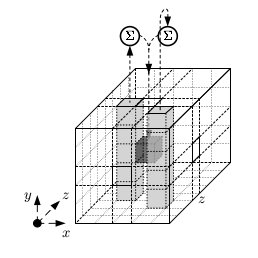
\includegraphics[scale=0.5]{keccaktheta.jpg}
  %\end{center}
  %\caption{$\theta$ applied to a single row\footnotemark}
  %\label{fig:lab}
%\end{figure}
%\footnotetext[23]{Guido Bertoni, Joan Daemen, Micha\"{e}l Peeters, and Gilles Van Assche. The keccak 
%reference. http://keccak.noekeon.org/Keccak-reference-3.0.pdf, January 2011.}
%\end{frame}

%\begin{frame}
%\frametitle{$\rho$ step}
%\begin{figure}[h]
  %\begin{center}
    %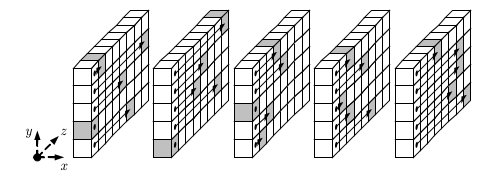
\includegraphics[scale=0.5]{keccakrho.jpg}
  %\end{center}
  %\caption{$\rho$ transformation applied to lanes\footnotemark}
  %\label{fig:lab}
%\end{figure}
%\footnotetext[24]{Guido Bertoni, Joan Daemen, Micha\"{e}l Peeters, and Gilles Van Assche. The keccak 
%reference. http://keccak.noekeon.org/Keccak-reference-3.0.pdf, January 2011.}
%\end{frame}

%\begin{frame}
%\frametitle{$\pi$ step}
%\begin{figure}[h]
  %\begin{center}
    %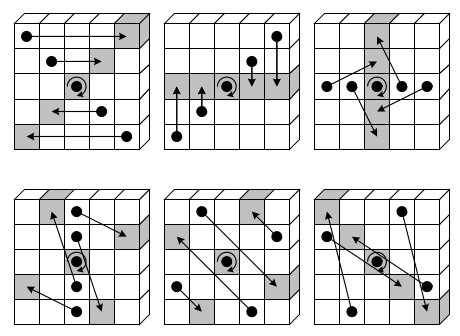
\includegraphics[scale=0.35]{keccakpi.jpg}
  %\end{center}
  %\caption{$\pi$ applied to a single slice\footnotemark}
  %\label{fig:lab}
%\end{figure}
%\footnotetext[25]{Guido Bertoni, Joan Daemen, Micha\"{e}l Peeters, and Gilles Van Assche. The keccak 
%reference. http://keccak.noekeon.org/Keccak-reference-3.0.pdf, January 2011.}
%\end{frame}

%\begin{frame}
%\frametitle{$\chi$ step}
%\begin{figure}[h]
  %\begin{center}
    %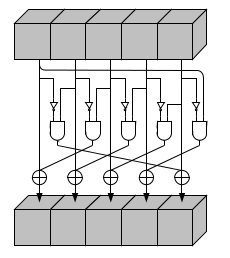
\includegraphics[scale=0.35]{keccakchi.jpg}
  %\end{center}
  %\caption{$\chi$ applied to a single row.\footnotemark}
  %\label{fig:lab}
%\end{figure}
%\footnotetext[26]{Guido Bertoni, Joan Daemen, Micha\"{e}l Peeters, and Gilles Van Assche. The keccak 
%reference. http://keccak.noekeon.org/Keccak-reference-3.0.pdf, January 2011.}
%\end{frame}

\begin{frame}
\frametitle{$\iota$ step}
\begin{itemize}
\item The round constants are given by
\begin{center}$RC[i_{r}][0][0][2^{j} - 1] = rc[j + 7i_{r}]$ for all $ 0 \leq j \leq l$,\end{center}
\item $rc[t] = (x^{t} \thickspace mod \thickspace x^{8} + x^{6} + x^{5} + x^{4} + 1)$ mod x in GF(2)[$x$]
\end{itemize}
\end{frame}

\subsection{BLAKE}

\begin{frame}
\frametitle{Properties of BLAKE hash function}
\begin{table}[h]
  \begin{center}
    \begin{tabular}{ *{6}{c} } \hline
      Algorithm & Word & Message    & Block & Digest & Salt \\ \hline
      BLAKE-224 & 32   & $< 2^{64}$  & 512   & 224    & 128  \\
      BLAKE-256 & 32   & $< 2^{64}$  & 512   & 256    & 128  \\
      BLAKE-384 & 64   & $< 2^{128}$ & 1024  & 384    & 256  \\
      BLAKE-512 & 64   & $< 2^{128}$ & 1024  & 512    & 256  \\ \hline
    \end{tabular}
    \caption{Specification of available input, output, block and salt sizes for various BLAKE hash functions,
    size in bits. \footnotemark}
  \end{center}
\end{table}
\footnotetext[11]{Jean-Philippe Aumasson, Luca Henzen, Willi Meier, and Raphael C.-W. Phan. Blake.
http://www.131002.net/blake/blake.pdf, April 2012.}
\end{frame}

\begin{frame}
\frametitle{BLAKE construction}
BLAKE is built on HAIFA (HAsh Iterative FrAmework) structure \footnotemark which is an improved version of 
Merkle-Damg\.{a}rd function.
\begin{figure}[h]
  \begin{center}
    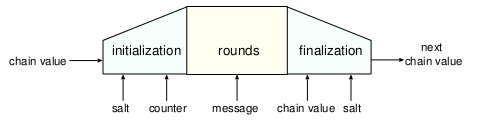
\includegraphics[scale=0.5]{blakelocalwidepipeconstruction.jpg}
  \end{center}
  \caption{Local wide construction of BLAKE's compression function\footnotemark}
  \label{fig:seq}
\end{figure}
\footnotetext[12]{Eli Biham and Orr Dunkelman. A framework for iterative hash functions - haifa.
Cryptology ePrint Archive, Report 2007/278, 2007.}
\footnotetext[13]{Jean-Philippe Aumasson, Luca Henzen, Willi Meier, and Raphael C.-W. Phan. Blake.
http://www.131002.net/blake/blake.pdf, April 2012.}
\end{frame}

\begin{frame}
\frametitle{Padding rule}
\begin{itemize}
\item For variant producing digest size 224, 256 input message is padded with '1' followed by '0' bits,
so that length is 447 modulo 512. Followed by bit '1', and 64 bit unsigned big endian representation 
of block length. 
\item For variant producing digest size 384, 512 input message is padded by bit '1', followed by '0' bits
till length is 895 modulo 1024. Followed by bit '1', and 128 bit unsigned big endian representation of 
block length in bits.
\end{itemize}
\end{frame}

\begin{frame}[fragile]
\frametitle{Compression algorithm}
  \begin{algorithm}[H]
  \begin{algorithmic}[1]
    \State $ h^{0} \gets IV $
    \For {$i = 0,\dots, N - 1$}
      \State $h^{i+1} \gets compress(h^{i}, m^{i}, s, l^{i})$
    \EndFor
    \State\Return{$h^{N}$}
  \end{algorithmic}
  \caption[BLAKE Compression]{BLAKE Compression procedure\footnotemark}
  \label{alg:seq}
  \end{algorithm}
  \footnotetext[14]{Jean-Philippe Aumasson, Luca Henzen, Willi Meier, and Raphael C.-W. Phan. Blake.
http://www.131002.net/blake/blake.pdf, April 2012.}
\end{frame}

\begin{frame}
\frametitle{Initialization of the state}
\begin{center}
$\begin{pmatrix} v_{0} & v_{1} & v_{2} & v_{3} \\ v_{4} & v_{5} & v_{6} & v_{7} \\
                 v_{8} & v_{9} & v_{10} & v_{11} \\ v_{12} & v_{13} & v_{14} & v_{15}\end{pmatrix} 
\gets
\begin{pmatrix} h_{0} & h_{1} & h_{2} & h_{3} \\ h_{4} & h_{5} & h_{6} & h_{7} \\
   s_{0} \oplus c_{0} & s_{1} \oplus c_{1} & s_{2} \oplus c_{2} & s_{3} \oplus c_{3} \\ 
   t_{0} \oplus c_{4} & t_{0} \oplus c_{5} & t_{1} \oplus c_{6} & t_{1} \oplus c_{7} \end{pmatrix}$
\end{center}
After initialization the matrix is operated for 14 or 16 rounds depending on version, on the following 
groups represented as $G_{i}(a, b, c, d)$
\begin{table}
  \begin{center}
    \begin{tabular}{ *{3}{c}}
    $ G_{0}(v_{0}, v_{8}, v_{12})$ & $G_{1}(v_{1}, v_{5}, v_{9}, v_{13})$ & $G_{2}(v_{2}, v_{6}, v_{10}, v_{14})$ \\
    $G_{3}(v_{3}, v_{7}, v_{11}, v_{15}) $ & $G_{4}(v_{0}, v_{5}, v_{10}, v_{15})$ & $G_{5}(v_{1}, v_{6}, v_{11}, v_{12})$ \\
    $G_{6}(v_{2}, v_{7}, v_{8}, v_{13})$ & $G_{7}(v_{3}, v_{4}, v_{9}, v_{14})$
    \end{tabular}
  \end{center}
\end{table}
\end{frame}

\begin{frame}
\frametitle{BLAKE permutation operation for 224 and 256 variant}
$a \gets a + b + (m_{\sigma_{r}(2i)} \oplus c_{\sigma_{r}(2i + 1)}) $ \\
$d \gets (d \oplus a) \ggg 16$ \\
$c \gets c + d$ \\
$b \gets (b \oplus c) \ggg 12$ \\
$a \gets a + b + (m_{\sigma_{r}(2i + 1)} \oplus c_{\sigma_{r}(2i)})$ \\
$d \gets (d \oplus a) \ggg 8$ \\
$c \gets c + d$ \\
$b \gets (b \oplus c) \ggg 7$ \\ 
\noindent\rule{10cm}{0.4pt} \\
\vspace{1mm}
+ addition in modulo $2^{32}$ \\
$\ggg k$ rotate to right by k bits \\
$\oplus$ bitwise XOR \\
r permutation round \\
i is from $G_{i}$
\end{frame}

\begin{frame}
\frametitle{Permutation round selection, $\sigma$ function\footnotemark}
  \resizebox{\linewidth}{!} {
    \begin{tabular}{ c| *{16}{c}} \hline
      $\sigma_{0}$ & 0  & 1  & 2  & 3  & 4  & 5  & 6  & 7  & 8  & 9  & 10 & 11 & 12 & 13 & 14 & 15 \\
      $\sigma_{1}$ & 14 & 10 & 4  & 8  & 9  & 15 & 13 & 6  & 1  & 12 & 0  & 2  & 11 & 7  & 5  & 3  \\
      $\sigma_{2}$ & 11 & 8  & 12 & 0  & 5  & 2  & 15 & 13 & 10 & 14 & 3  & 6  & 7  & 1  & 9  & 4  \\
      $\sigma_{3}$ & 7  & 9  & 3  & 1  & 13 & 12 & 11 & 14 & 2  & 6  & 5  & 10 & 4  & 0  & 15 & 8  \\
      $\sigma_{4}$ & 9  & 0  & 5  & 7  & 2  & 4  & 10 & 15 & 14 & 1  & 11 & 12 & 6  & 8  & 3  & 13 \\
      $\sigma_{5}$ & 2  & 12 & 6  & 10 & 0  & 11 & 8  & 3  & 4  & 13 & 7  & 5  & 15 & 14 & 1  & 9  \\
      $\sigma_{6}$ & 12 & 5  & 1  & 15 & 14 & 13 & 4  & 10 & 0  & 7  & 6  & 3  & 9  & 2  & 8  & 11 \\
      $\sigma_{7}$ & 13 & 11 & 7  & 14 & 12 & 1  & 3  & 9  & 5  & 0  & 15 & 4  & 8  & 6  & 2  & 10 \\
      $\sigma_{8}$ & 6  & 15 & 14 & 9  & 11 & 3  & 0  & 8  & 12 & 2  & 13 & 7  & 1  & 4  & 10 & 5  \\
      $\sigma_{9}$ & 10 & 2  & 8  & 4  & 7  & 6  & 1  & 5  & 15 & 11 & 9  & 14 & 3  & 12 & 13 & 0  \\ \hline
    \end{tabular}
  }
  \footnotetext[15]{Jean-Philippe Aumasson, Luca Henzen, Willi Meier, and Raphael C.-W. Phan. Blake.
http://www.131002.net/blake/blake.pdf, April 2012.}
\end{frame}

\begin{frame}
\frametitle{BLAKE permutation operation for 384 and 512 variant}
$a \gets a + b + (m_{\sigma_{r}(2i)} \oplus c_{\sigma_{r}(2i + 1)})$ \\
$d \gets (d \oplus a) \ggg 32$ \\
$c \gets c + d$ \\
$b \gets (b \oplus c) \ggg 25$ \\
$a \gets a + b + (m_{\sigma_{r}(2i + 1)} \oplus c_{\sigma_{r}(2i)})$ \\
$d \gets (d \oplus a) \ggg 16$ \\
$c \gets c + d$ \\
$b \gets (b \oplus c) \ggg 11$ \\
\noindent\rule{10cm}{0.4pt} \\
\vspace{1mm}
+ addition in modulo $2^{64}$ \\
\end{frame}

\begin{frame}
\frametitle{Finalization}
$h'_{0} \gets h_{0} \oplus s_{0} \oplus v_{0} \oplus v_{8}$ \\
$h'_{1} \gets h_{1} \oplus s_{1} \oplus v_{1} \oplus v_{9}$ \\
$h'_{2} \gets h_{2} \oplus s_{2} \oplus v_{2} \oplus v_{10}$ \\
$h'_{3} \gets h_{3} \oplus s_{3} \oplus v_{3} \oplus v_{11}$ \\
$h'_{4} \gets h_{4} \oplus s_{0} \oplus v_{4} \oplus v_{12}$ \\
$h'_{5} \gets h_{5} \oplus s_{1} \oplus v_{5} \oplus v_{13}$ \\
$h'_{6} \gets h_{6} \oplus s_{2} \oplus v_{6} \oplus v_{14}$ \\
$h'_{7} \gets h_{7} \oplus s_{3} \oplus v_{7} \oplus v_{15}$ \\
\end{frame}

\subsection{Gr{\o}stl}

\begin{frame}
\frametitle{Padding}
\begin{itemize}
\item The message is split into blocks of 512 bits for variants of digest size upto 256 bits; and into 1024 bit
block for variant of digest size above 256 bits.
\item Bit '1' is appended, then $ w = -N - 65 \thickspace mod \thickspace l $, 0 bits are appended; followed by
64 bit representation of $(N + w + 65) / l $.
\item Due to encoding of message in padded block, the maximum size of message for short variants is $2^{73}-577$
bits, and that for variants above 256 is $2^{74}-1089$bits.
\end{itemize}
\end{frame}

\begin{frame}
\frametitle{Initial values and rounds \footnotemark}
\begin{table}[h]
  \begin{center}
    \begin{tabular}{ *{3}{c} } \hline
      Permutations            & Digest size & Recommended value of r \\ \hline
      $P_{512}$ and $Q_{512}$   & 8 - 256     & 10 \\
      $P_{1024}$ and $Q_{1024}$ & 264 - 512   & 14 \\ \hline 
    \end{tabular}
    \caption{Recommended number of rounds}
  \end{center}
\end{table}

\begin{table}[h]
  \begin{center}
    \begin{tabular}{ *{2}{c} } \hline
      n   & $iv_{n}$         \\ \hline
      224 & 00 $\dots$ 00 00 e0 \\
      256 & 00 $\dots$ 00 01 00 \\
      384 & 00 $\dots$ 00 01 80 \\
      512 & 00 $\dots$ 00 02 00 \\ \hline
    \end{tabular}
  \caption{Initial values for Gr{\o}stl-n function.}
  \end{center}
\end{table}
\footnotetext[16]{S{\o}ren Steffen Thomsen, Martin Schl\"{a}ffer, Christian Rechberger, Florian Mendel,
Krystian Matusiewicz, Lars R. Knudsen, and Praveen Gauravaram. Grøstl - a sha-3
candidate version 2.0.1. http://www.groestl.info/Groestl.pdf, March 2011.}
\end{frame}

\begin{frame}
\frametitle{Hashing the message}
After padding, the message is broken to blocks, and processed sequentially. An initial $h_{0}$ = iv is defined.
\begin{center}$ h_{i}\gets f(h_{i-1}, m_{i})\thickspace for \thickspace i = 1,\ldots, t.$\end{center}
\begin{figure}
  \begin{center}
    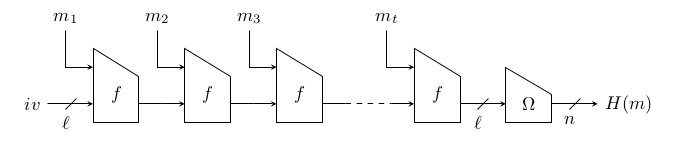
\includegraphics[scale=0.5]{groestlhashfunction.jpg}
  \end{center}
  \caption{Gr{\o}stl hash function \footnotemark}
  \label{fig:lab}
\end{figure}
\footnotetext[17]{S{\o}ren Steffen Thomsen, Martin Schl\"{a}ffer, Christian Rechberger, Florian Mendel,
Krystian Matusiewicz, Lars R. Knudsen, and Praveen Gauravaram. Grøstl - a sha-3
candidate version 2.0.1. http://www.groestl.info/Groestl.pdf, March 2011.}
\end{frame}

\begin{frame}
\frametitle{Input mapping}
Mapping of the input bytes to the state in following order. \\
\vspace{3mm}
$\begin{bmatrix}
  00 & 08 & 10 & 18 & 20 & 28 & 30 & 38 \\
  01 & 09 & 11 & 19 & 21 & 29 & 31 & 39 \\
  02 & 0a & 12 & 1a & 22 & 2a & 32 & 3a \\
  03 & 0b & 13 & 1b & 23 & 2b & 33 & 3b \\
  04 & 0c & 14 & 1c & 24 & 2c & 34 & 3c \\
  05 & 0d & 15 & 1d & 25 & 2d & 35 & 3d \\
  06 & 0e & 16 & 1e & 26 & 2e & 36 & 3e \\
  07 & 0f & 17 & 1f & 27 & 2f & 37 & 3f
\end{bmatrix}$
\end{frame}

\begin{frame}
\frametitle{Permutation f function}
\begin{center}$f(h, m) = P(h \oplus m) \oplus Q(m) \oplus h.$\end{center}
\begin{figure}[h]
  \begin{center}
    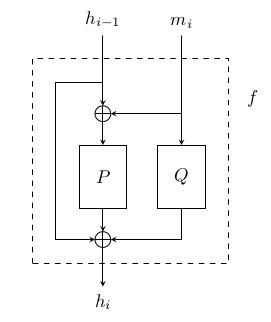
\includegraphics[scale=0.5]{groestlPQfunction.jpg}
  \end{center}
  \caption{Compression functions, where P and Q are $l-bit$ permutations \footnotemark}
  \label{fig:lab}
\end{figure}
\footnotetext[18]{S{\o}ren Steffen Thomsen, Martin Schl\"{a}ffer, Christian Rechberger, Florian Mendel,
Krystian Matusiewicz, Lars R. Knudsen, and Praveen Gauravaram. Grøstl - a sha-3
candidate version 2.0.1. http://www.groestl.info/Groestl.pdf, March 2011.}
\end{frame}

\begin{frame}
\frametitle{Omega truncate function}
The $\Omega$ function consists of a $trunc_{n}(x)$ that outputs only the trailing n bits of input x.
\begin{center}$\Omega(x) = trunc_{n}( P(x) \oplus x ).$\end{center}
\begin{figure}[h]
  \begin{center}
    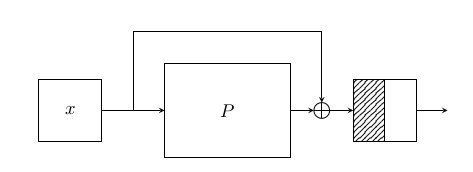
\includegraphics[width=4.5in]{groestlomegafunction.jpg}
  \end{center}
  \caption{Omega truncation function \footnotemark}
  \label{fig:lab}
\end{figure}
\footnotetext[19]{S{\o}ren Steffen Thomsen, Martin Schl\"{a}ffer, Christian Rechberger, Florian Mendel,
Krystian Matusiewicz, Lars R. Knudsen, and Praveen Gauravaram. Grøstl - a sha-3
candidate version 2.0.1. http://www.groestl.info/Groestl.pdf, March 2011.}
\end{frame}

\begin{frame}
\frametitle{Contents of P and Q function}
The P and Q functions are represented by a round, with slight variation in variables they operate.
\begin{center}$ R = MixBytes \cdot ShiftBytes \cdot SubBytes \cdot AddRoundConstant $ \end{center}
\end{frame}

\begin{frame}
\frametitle{Add Round Constant}
$A \gets A \oplus C[i]$ where A is state matrix and C is constant matrix.
$ P_{1024}: C[i] = \begin{bmatrix}
  00 \oplus i & 10 \oplus i & 20 \oplus i \ldots f0 \oplus i \\
  00          & 00          & 00          \dots  00          \\
  \vdots      & \vdots      & \vdots      \dots  \vdots      \\
\end{bmatrix}$

and 

$Q_{1024}: C[i] = \begin{bmatrix}
  ff          & ff          & ff          \dots ff          \\
  \vdots      & \vdots      & ff          \dots ff          \\
  ff \oplus i & ef \oplus i & df \oplus i \dots 0f \oplus i
\end{bmatrix}$
\end{frame}

\begin{frame}
\frametitle{Substitute byte}
$a_{i,j} \gets S( a_{i,j}),  0 \leq i < 8, 0 \leq j < v.$ 
\resizebox{\linewidth}{!} {
    \begin{tabular}{ c | *{16}{c}}
     & 00 & 01 & 02 & 03 & 04 & 05 & 06 & 07 & 08 & 09 & 0a & 0b & 0c & 0d & 0e & 0f \\ \hline
  00 & 63 & 7c & 77 & 7b & f2 & 6b & 6f & c5 & 30 & 01 & 67 & 2b & fe & d7 & ab & 76 \\ 
  10 & ca & 82 & c9 & 7d & fa & 59 & 47 & f0 & ad & d4 & a2 & af & 9c & a4 & 72 & c0 \\
  20 & b7 & fd & 93 & 26 & 36 & 3f & f7 & cc & 34 & a5 & e5 & f1 & 71 & d8 & 31 & 15 \\
  30 & 04 & c7 & 23 & c3 & 18 & 96 & 05 & 9a & 07 & 12 & 80 & e2 & eb & 27 & b2 & 75 \\
  40 & 09 & 83 & 2c & 1a & 1b & 6e & 5a & a0 & 52 & 3b & d6 & b3 & 29 & e3 & 2f & 84 \\
  50 & 53 & d1 & 00 & ed & 20 & fc & b1 & 5b & 6a & cb & be & 39 & 4a & 4c & 58 & cf \\
  60 & d0 & ef & aa & fb & 43 & 4d & 33 & 85 & 45 & f9 & 02 & 7f & 50 & 3c & 9f & a8 \\
  70 & 51 & a3 & 40 & 8f & 92 & 9d & 38 & f5 & bc & b6 & da & 21 & 10 & ff & f3 & d2 \\
  80 & cd & 0c & 13 & ec & 5f & 97 & 44 & 17 & c4 & a7 & 7e & 3d & 64 & 5d & 19 & 73 \\
  90 & 60 & 81 & 4f & dc & 22 & 2a & 90 & 88 & 46 & ee & b8 & 14 & de & 5e & 0b & db \\
  a0 & e0 & 32 & 3a & 0a & 49 & 06 & 24 & 5c & c2 & d3 & ac & 62 & 91 & 95 & e4 & 79 \\
  b0 & e7 & c8 & 37 & 6d & 8d & d5 & 4e & a9 & 6c & 56 & f4 & ea & 65 & 7a & ae & 08 \\
  c0 & ba & 78 & 25 & 2e & 1c & a6 & b4 & c6 & e8 & dd & 74 & 1f & 4b & bd & 8b & 8a \\
  d0 & 70 & 3e & b5 & 66 & 48 & 03 & f6 & 0e & 61 & 35 & 57 & b9 & 86 & c1 & 1d & 9e \\
  e0 & e1 & f8 & 98 & 11 & 69 & d9 & 8e & 94 & 9b & 1e & 87 & e9 & ce & 55 & 28 & df \\
  f0 & 8c & a1 & 89 & 0d & bf & e6 & 42 & 68 & 41 & 99 & 2d & 0f & b0 & 54 & bb & 16 \\
  \end{tabular}
  }
\end{frame}

\begin{frame}
\frametitle{Shift byte}
\begin{figure}[h]
  \begin{center}
    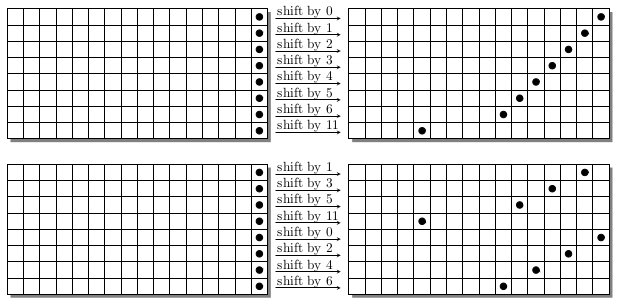
\includegraphics[scale=0.5]{groestl1024shift.jpg}
  \end{center}
  \caption{ShiftBytes transformation of permutation $P_{1024}$(top) and $Q_{1024}$(bottom)\footnotemark}
  \label{fig:lab}
\end{figure}
\footnotetext[20]{S{\o}ren Steffen Thomsen, Martin Schl\"{a}ffer, Christian Rechberger, Florian Mendel,
Krystian Matusiewicz, Lars R. Knudsen, and Praveen Gauravaram. Grøstl - a sha-3
candidate version 2.0.1. http://www.groestl.info/Groestl.pdf, March 2011.}
\end{frame}

\begin{frame}
\frametitle{Mix byte}
$ A \gets B \times A$ \\
B is a finite field over $\mathbb{F}_{256}$, 
defined over $\mathbb{F}_{2}$ by polynomial $x^{8} \oplus x^{4} \oplus x^{3} \oplus x \oplus 1$. \\
\vspace{3mm}
$B = \begin{bmatrix}
02 & 02 & 03 & 04 & 05 & 03 & 05 & 07 \\
07 & 02 & 02 & 03 & 04 & 05 & 03 & 05 \\
05 & 07 & 02 & 02 & 03 & 04 & 05 & 03 \\
03 & 05 & 07 & 02 & 02 & 03 & 04 & 05 \\
05 & 03 & 05 & 07 & 02 & 02 & 03 & 04 \\
04 & 05 & 03 & 05 & 07 & 02 & 02 & 03 \\
03 & 04 & 05 & 03 & 05 & 07 & 02 & 02 \\
02 & 03 & 04 & 05 & 03 & 05 & 07 & 02 \\
\end{bmatrix}$
\end{frame}

\section{Related work, hypothesis based on hill climbing}

%\subsection{Rotational cryptanalysis of reduced round Keccak}

%\begin{frame}
%\frametitle{Rotational cryptanalysis in ARX}
%\begin{itemize}
%\item Rotational cryptanalysis that studies propogation of rotational pair throug a primitive, is used on 
%reduced version of Threefish, a core of Skein\footnotemark.
%\item Pair of two 1600-bit states $(A, A^{\leftarrow})$ are called rotational pair when each lane in 
%state $A^{\leftarrow}$ is created by bitwise rotation of operation of corresponding lane in state $A$
%\footnotemark.
%\end{itemize}
%\footnotetext[27]{Dmitry Khovratovich and Ivica Nikoli. Rotational cryptanalysis of arx. In Seokhie
%Hong and Tetsu Iwata, editors, Fast Software Encryption, volume 6147 of Lecture
%Notes in Computer Science, pages 333–346. Springer Berlin Heidelberg, 2010.}
%\footnotetext[28]{Pawe{\l} Morawiecki, Josef Pieprzyk, and Marian Srebrny. Rotational cryptanalysis of
%round-reduced keccak. Cryptology ePrint Archive, Report 2012/546, 2012. http://eprint.iacr.org/2012/546.pdf.}
%\end{frame}

%\begin{frame}
%\frametitle{Definitions}
%\begin{enumerate}
%\item Set $S_n$ is a set of $2^{1600}$ pairs of states which are created by an operation of KECCAK-f[1600] 
%applied to all possible rotational pairs.
%\item Probability $p^{n}_{(x, y, z)}$ is the probability for pair of states $(A, A^{\leftarrow})$ randomly 
%selected from the set $S_n$ we have $A_{(x, y, z)} = A^{\leftarrow}_{(x, y, z + n)}$.
%\item Given probability distribution $\mathcal{D}_n$ that assigns probability $\frac{1}{n!}$ for each 
%$p \in \mathcal{P}_n$. A permutation is random, if chosen from $\mathcal{D}_n$.
%\end{enumerate}
%\end{frame}

%\begin{frame}
%\frametitle{Probability distribution and distinguisher}
%\begin{itemize}
%\item Random permutation $p^n_{(x, y, z)}$ should follow binomial distribution $\mathcal{B}(t, s)$ that is equal
%to 0.5. Experimental values are supposed to fall within range of $0.5t\pm2\sigma$ with 95\% confidence interval.
%\item A 4 round rotational for Keccak was built, and 10,000 samples selected from it. $p^{54}_{(4, 4, 14)} = 0.5625$
%had highest deviation, and the mean was 5682. Mean should not have exceeded from range of 
%$\mathcal{B}(10000, 0.5)$ which is 5000$\pm$2.5.
%\item After four rounds however, $p^n_{(x, y, z)} = 0.5$, and hence the distinguisher cannot be directly extended.
%\end{itemize}
%\end{frame}

%\begin{frame}
%\frametitle{Extend probabilities beyond 4 round Keccak}
%\begin{enumerate}
%\item Find probability that relation between two pairs of states $(A_{(x, y, z)}, A^{\leftarrow}_{(x, y, z+n)})$ 
%and $(A_{(x, y', z)}, A^{\leftarrow}_{(x, y'', z+n)})$ are observed, that should follow distribution 
%$\mathcal{B}(10000, 0.5)$.
%\item Bit wise operations like NOT, or rotation in Keccak do not affect the probabilities, but AND and XOR do.
%\item AND operation $P_{out} = \frac{1}{2}(p_{a} + p_{b} - p_{a} p_{b})$ \footnotemark
%\item XOR operation $P_{out} = p_{a} + p_{b} - 2 p_{a} p_{b}$
%\end{enumerate}
%\footnotetext[29]{Pawe{\l} Morawiecki, Josef Pieprzyk, and Marian Srebrny. Rotational cryptanalysis of
%round-reduced keccak. Cryptology ePrint Archive, Report 2012/546, 2012. http://eprint.iacr.org/2012/546.pdf.}
%\end{frame}

%\begin{frame}
%\frametitle{Extending probability beyond 4 rounds}
%\begin{itemize}
%\item $p^{63}_{(2, 1, 37)}$ and $p^{63}_{(2, 2, 37)}$ have the highest deviation from 0.5 at end of fourth round.
%\item Probability that they are in the same relation is given by $p^n_{(x, y, z)} \dot p^n_{(x, y'', z)} + (1 - p^n_{(x, y, z)})
%(1 - p^n_{(x, y, z)})$ which is around 0.499024.
%\item To observe bias generate 403,000,000 samples obtained by selecting $\in$ error at 0.05 in Chernoff inequality \\
%\[ m \geq \frac{1}{(P_c - 0.5)^2} \ln \frac{1}{\sqrt \in}\]
%\end{itemize}
%\end{frame}

%\begin{frame}
%\frametitle{Extending probability beyond 4 rounds}
  %\begin{algorithm}[H]
  %\begin{algorithmic}[1]
    %\State Generate 403,000,000 rotational pairs.
    %\ForAll{403,000,000 rotational pairs}
      %\State Run Keccak for 5 rounds on states $A$ and $A^{\leftarrow}$.
      %\If{$(A_{(1, 2, 43)} \oplus A^{\leftarrow}_{(1, 2, 44)} \oplus A_{(2, 0, 16)} \oplus A^{\leftarrow}_{(2, 0, 17)} = 0)$}
      %\State mean := mean + 1
      %\EndIf
    %\EndFor
    %\State \Return mean
  %\end{algorithmic}
  %\caption[Find pair probabililty]{Find pair probabililty\footnotemark}
  %\label{alg:seq}
  %\end{algorithm}
%\footnotetext[30]{Pawe{\l} Morawiecki, Josef Pieprzyk, and Marian Srebrny. Rotational cryptanalysis of
%round-reduced keccak. Cryptology ePrint Archive, Report 2012/546, 2012. http://eprint.iacr.org/2012/546.pdf.}
%\end{frame}

%\begin{frame}
%\frametitle{Distinguisher Keccak and find preimage}
%\begin{enumerate}
%\item Mean for $\mathcal{B}(403000000, 0.5)$ with the standard deviation has range of 201,500,000$\pm$2.10037, 
%but experimentally from above procedure it comes to around 201,450,503.
%\item For primage, unknown message with cyclical property like 4 0's followed by 4 1's, alternatively of 512 bits
%is chosen. There are 256 possible message for rotational counterpart.
%\item A rotational counterpart of the preimage is searched, that reduces complexity of random search.
%\end{enumerate}
%\end{frame}

%\begin{frame}[allowframebreaks]
%\frametitle{Preimage for 3 rounds of Keccak \footnotemark}
%\begin{algorithmic}[1]
  %\State Guess first 8 lanes of $A^{\leftarrow}$
  %\State Run Keccak-f[1600] for 3 rounds on state $A^{\leftarrow}$
  %\For {for n:= 0 to n \textless 64}
    %\State candidate := true
    %\For{10 sets of cordinates $(x, y, z)$ being on list created on precomputation}
      %\If{$(p^n_{(x, y, z)} = 1)$ and $(A_{(x, y, z)} = A^{\leftarrow}_{(x, y, z)})$}
        %\State candidate := false
      %\EndIf
      %\If{$(p^n_{(x, y, z)} = 0)$ and $(A_{(x, y, z)} \neq A^{\leftarrow}_{(x, y, z)})$}
        %\State candidate := false
      %\EndIf
    %\EndFor
    %\If{ candidate = true }
      %\State Rotate the guessed state by n bits
      %\State Verify input to Keccak, that runs for 3 rounds.
    %\EndIf
  %\EndFor
%\end{algorithmic}
%\footnotetext[32]{Pawe{\l} Morawiecki, Josef Pieprzyk, and Marian Srebrny. Rotational cryptanalysis of
%round-reduced keccak. Cryptology ePrint Archive, Report 2012/546, 2012. http://eprint.iacr.org/2012/546.pdf.}
%\end{frame}

%\begin{frame}
%\frametitle{How the search is better than random search}
%\begin{enumerate}
%\item For guessing 512 bits, from 64 rotational pairs, the probability for guessing rotational counterpart
%is $A^{\leftarrow}$ is $2^{-512} \cdot 64 = 2^{-506}$.
%\item There are $2^{256}$ messages of the cyclic pattern, and 10 sets of $(x, y, z)$ cordinates for each of
%the rotational number.
%\item The probability of the candidate having $p^n_{(x, y, z)}$ similar to that on list is $2^{-10}$. 
%So $2^{512} / 2^{10} = 2^{502}$ number of checks are required at most.
%\item You can extend this to 4 rounds of Keccak, but will have to drop the $\iota$, round constant addition
%round, since it makes $p^n_{(x, y, z)} \neq 0, 1$.
%\end{enumerate}
%\end{frame}

\subsection{Hill climbing}

\begin{frame}
\frametitle{Collisions}
\begin{enumerate}
\item Collision in hash function, is when we have two different messages hashing to the same value, using
same initial value.
\item Full collision is when all the bits agree in the hash output for two different messages.
\item Semi-free start collision is where you change the initial value and obtain collisions for two 
different message.
\end{enumerate}
\end{frame}

\begin{frame}
\frametitle{Near collisions found with hill climbing}
\begin{enumerate}
\item A $\epsilon / n $ bit near collision for hash function for two messages $M_{1}$ and $M_{2}$, where 
$M_{1} \neq M_{2}$ is defined as $HW( h( M_{1}, CV ) \oplus h( M_{2}, CV ) ) = n - \epsilon $.
\item Near collisions in which more than 75\% of the bits were same for two different messages, were found 
for reduced rounds of BLAKE-32, Hamsi-256 and JH.
\item Hill Climbing starts with a random candidate, and then choosing a random successor that has a better
fit to the solution. Ideally $HW( h(M, CV) \oplus h(M, CV + \delta) ) = n / 2 $ where $\delta$ is n-bit 
vector with small Hamming weight.
\end{enumerate}
\end{frame}

\begin{frame}
\frametitle{Table of effort to find near collisions with random search}
\begin{table}
  \begin{center}
    \begin{tabular}{ | c | c | } \hline
      $\epsilon / n $            & Complexity $( \approx )$ \\ \hline
      128/256, 256/512, 512/1024 & $2^{4}$ \\ \hline
      151/256, 287/512, 553/1024 & $2^{10}$ \\ \hline
      166/256, 308/512, 585/1024 & $2^{20}$ \\ \hline
      176/256, 323/512, 606/1024 & $2^{30}$ \\ \hline
      184/256, 335/512, 623/1024 & $2^{40}$ \\ \hline
      191/256, 345/512, 638/1024 & $2^{50}$ \\ \hline
      197/256, 354/512, 651/1024 & $2^{60}$ \\ \hline
    \end{tabular}
    \caption{Approximate complexity to find a $\epsilon / n$-bit near collision by generic random search
    \footnotemark}
  \end{center}
\end{table}
\footnotetext[24]{Meltem S\"{o}nmez Turan and Erdener Uyan. Practical near-collisions for reduced round blake, 
fugue, hamsi and jh. Second SHA-3 conference, August 2010. 
http://csrc.nist.gov/groups/ST/hash/sha-3/Round2/Aug2010/documents/papers/TURAN\_Paper\_Erdener.pdf.}
\end{frame}

\begin{frame}
\frametitle{How hill climbing works}
\begin{enumerate}
\item Hill climbing algorithm will be to minimize the function 
$f_{M_{1}, M_{2}}(x) = HW( h(M_{1}, x) \oplus h(M_{2}, x) )$.
\item CV is chosen as any random chaining value. Then the set of k-bit neighbours for the CV are created
$S^{k}_{CV} = \{ x \in \{0, 1\}^{n} \mid HW( CV \oplus x ) \leq k \}$.
\item Hill climbing is used to obtain k-optimum condition from k-bit neighbours 
$f_{M_{1}, M_{2}} (CV) =  \min\limits_{x \in S^{k}_{CV}} f_{M_{1}, M_{2}} (x)$.
\end{enumerate}
\end{frame}

\begin{frame}{fragile}
\frametitle{Hill Climbing algorithm}
\begin{algorithm}[H]
  \begin{algorithmic}[1]
    \State Randomly select CV
    \State $f_{best} = f_{M_{1}, M_{2}}(CV)$
    \While {(CV is not k-opt)}
    \State CV = x such that $x \in S^{k}_{CV}$ with $f(x) < f(best)$
    \State $f_{best} = f_{M_{1}, M_{2}}(CV)$
    \EndWhile
    \State \Return (CV, $f_{best}$)
  \end{algorithmic}
  \caption{Hill Climbing algorithm ($M_{1}, M_{2}, k$)}
\end{algorithm}
\end{frame}

\subsection{Other search algorithms}

\begin{frame}[allowframebreaks]
\frametitle{Simulated annealing}
  \begin{algorithmic}[1]
    \Function {Simulated-annealing}{$M_{1}, M_{2}, CV,$ schedule}
      \State current $\gets \thickspace CV$
      \For { t = 1 to $\infty$ }
        \State T $\gets$ schedule( t )
        \If { T = 0}
          \State \Return current
        \EndIf
        \State next $\gets$ a randomly selected successor from set $S^{k}_{current}$
        \State $\Delta E \gets  \thickspace f_{M_{1}, M_{2}}(current) - f_{M_{1}, M_{2}}(next)$
        \If { $\Delta$E $>$ 0 }
          \State current $\gets$ next
        \Else
          \State current $\gets$ next, with probability $e^{\Delta E / T}$
        \EndIf
      \EndFor
    \EndFunction
  \end{algorithmic}
\end{frame}

\begin{frame}[allowframebreaks]
\frametitle{Tabu search}
  \begin{algorithmic}[1]
    \Function {Tabu-search}{$TabuList_{size}, M_{1}, M_{2}, CV$}
      \State $S_{best}$ $\gets \thickspace CV$
      \State $TabuList \thickspace \gets$ null
      \While {$S_{best}$ not k-opt}
        \State CandidateList $\gets$ null
        \State $S_{neighbourhood} \gets S^{k}_{S_{best}}$
        \For { $S_{candidate} \in S_{best_{neighbourhood}}$}
          \If {($\lnot$ContainsAnyFeatures( $S_{candidate}, TabuList$ ))} 
            \State CandidateList $\gets$ $S_{candidate}$
          \EndIf
        \EndFor
        \State $S_{candidate}$ $\gets$ LocateBestCandidate( CandidateList )
        \If { Cost( $S_{candidate}$ ) $\leq$ Cost( $S_{best}$ ) }
          \State $S_{best} \gets S_{candidate}$
          \State $TabuList \gets$ featureDifferences$(S_{candidate}, S_{best})$
          \While { $TabuList >TabuList_{size}$ }
            \State DeleteFeature( $TabuList$ )
          \EndWhile
        \EndIf
      \EndWhile 
      \State \Return $S_{best}$
    \EndFunction
  \end{algorithmic}
\end{frame}

\begin{frame}[allowframebreaks]
\frametitle{Random selection}
  \begin{algorithmic}[1]
    \Function {Random-Selection}{$ M_{1}, M_{2}, CV,$ number\_of\_trials}
      \State current $\gets \thickspace CV$
      \State trial $\gets$ 0
      \While { trial $<$ number\_of\_trials }
        \State next $\gets$ randomly selected candidate from $S^{k}_{current}$
        \If { $f_{M_{1}, M_{2}}(next) - f_{M_{1}, M_{2}}(current) $ }
          \State current $\gets$ next
        \EndIf
      \EndWhile 
      \State \Return current
    \EndFunction
  \end{algorithmic}
\end{frame}

\subsection{Hypothesis}

\begin{frame}
\frametitle{Hypothesis}
\begin{itemize}
\item Reduced state Keccak, has better resistance to near collisions than BLAKE and Gr{\o}stl, for
search algorithms hill climbing, simulated annealing, tabu search and random selection.
\item Simulated annealing and tabu search, are better at finding near collisions compared to hill 
climbing and random selection.
\item State size has no effect on efficiency of Keccak permutation rounds.    
\end{itemize}
\end{frame}

\section{Experiment design}

\subsection{Input and output}

\begin{frame}
\frametitle{Input}
\begin{itemize}
\item The seed message is "The quick brown fox jumps over the lazy dog". 20 pairs are made from the
string, for each of the three categories start, middle and end.
\item The pair contains the original seed message and the seed message toggled for one bit. For each
category 20 bits are toggled. The bits are toggled at the start, middle and end of the seed string.
\item For input string $01100010\thickspace00011000$, then in input file 1.txt; pair will be made with this seed
string and ${\bf 1}1100010\thickspace00011000$, in file 2.txt the other  string will be 
$0{\bf 0}100010\thickspace00011000$.
\end{itemize}
\end{frame}

\begin{frame}
\frametitle{Input}
\begin{enumerate}
\item For the middle section, the bits are toggled to either side of the middle bit, in the string. For example
for seed string $01100010\thickspace00011000$, the file 1.txt will have seed and string 
$0110001{\bf 1}\thickspace00011000$, and file 2.txt will have modified string as 
$01100010\thickspace{\bf 1}0011000$.
\item For the ending section the bit toggling starts from the least significant bits, so for seed string
$01100010\thickspace00011000$, file 1.txt has updated string $01100010\thickspace0001100{\bf 1}$, and 
file 2.txt have updated string $01100010\thickspace000110{\bf 1}0$.
\end{enumerate}
\end{frame}

\begin{frame}
\frametitle{Output structure}
\begin{enumerate}
\item The output folder is arranged to have the results in the following way starting from the upper most
folder 
Output/chaining\_value/collision\_search/digest\_size/SHA3\_finalist/number\_of\_rounds/input\_category/output\_file.
\item The results for the input message pair of the respective file are inserted to corresponding output file.
Output for input file start/1.txt will be found in experiment parameter defined path and then start/1.txt
\end{enumerate}
\end{frame}

\begin{frame}
\frametitle{Ouput file}
\begin{enumerate}
\item The file contains 8 parameters, 3 each for either success or failure. Success is defined as finding near 
collision that is more than 65\% of the bits similar. The parameters are number of trials in success/failure,
total iterations, and average iterations.
\item The rest 2 are total iterations and average iterations. These iteration numbers are mostly useful for
hill climbing, since iterations for other algorithms are fixed.
\end{enumerate}
\end{frame}

\subsection{Chaining value and number of trials}

\begin{frame}
\frametitle{Number of trials and iterations}
\begin{enumerate}
\item The number of trials was initially kept at 128, but then increased to 256 to get more accurate numbers.
In each trial of experiment, the chaining value is randomly selected.
\item The iterations are the number of times that that algorithm has to loop through for its' operation. This is
chosen, over time required since differences in algorithm implementation may skew the time taken for finding
effectiveness of the search algorithm.
\end{enumerate}
\end{frame}

\begin{frame}
\frametitle{Chaining value and neighbourhood}
\begin{enumerate}
\item The chaining value length can be varied from 32, 64, 128, 256, 512 and 1024. We chose to do experiment
with 32 bit chaining value, and then 64 bit chaining value.
\item Other higher chaining value lengths were not tried, given the expensive time computation, and relatively
less success, in finding collisions.
\item k for k bit neighbourhood value is limited to less than equal to 2. Numbers above that are not optimal. 
\end{enumerate}
\end{frame}

\subsection{Demo}
\begin{frame}
\frametitle{Demo}
Demo
\end{frame}

\section{Observations}

\subsection{Implementation}

\begin{frame}
\frametitle{Observations on implementation}
\begin{itemize}
\item Use system or language representation of words like int and long, instead of array of bytes, made
it easier.
\item Java has signed representation of int and long. This should be considered when rotating blocks.
\item In Keccak the bits are ordered in little endian format, which is differnt that other general
implementation that take big endian.
\item During bitwise operation of byte or short datatype, Java will upcast the data to int and then
downcast result. This should be guarded against.
\end{itemize}
\end{frame}

\subsection{Average iterations}

\begin{frame}
\frametitle{Iterations for BLAKE, chaining value 32 bits}
\begin{table}
  \begin{center}
    \begin{tabular}{ | c | c | c | c | c | } \hline
     \multirow{2}{*}{Digest Size} & \multicolumn{4}{c|}{Rounds} \\ \cline{2-5}
                                  & 1    & 2   & 3   & 4   \\ \hline
     224                          & 803  & 891 & 886 & 883 \\ \hline
     256                          & 804  & 891 & 892 & 885 \\ \hline
     384                          & 1137 & 898 & 899 & 902 \\ \hline
     512                          & 1118 & 902 & 903 & 906 \\ \hline
    \end{tabular}
    \caption{Average iterations over all input cases for Hill Climbing for BLAKE for chaining value
    of bit length 32}
  \end{center}
\end{table}
\end{frame}

\begin{frame}
\frametitle{Iterations for BLAKE, chaining value 64 bits}
\begin{table}
  \begin{center}
    \begin{tabular}{ | c | c | c | c | } \hline
     \multirow{2}{*}{Digest Size} & \multicolumn{3}{ c|}{Rounds} \\ \cline{2-4}
                                  & 1    & 2    & 3    \\ \hline
     224                          & 4190 & 3465 & 3483 \\ \hline
     256                          & 4264 & 3456 & 3431 \\ \hline
     384                          & 3885 & 3515 & 3528 \\ \hline
     512                          & 3984 & 3535 & 3559 \\ \hline
    \end{tabular}
    \caption{Average iterations over all input cases for Hill Climbing for BLAKE for chaining value
    of bit length 64}
  \end{center}
\end{table}
\end{frame}

\begin{frame}
\frametitle{Iterations for Gr{\o}stl, chaining value 32 bits}
\begin{table}
  \begin{center}
    \begin{tabular}{ | c | c | c | c | c | } \hline
     \multirow{2}{*}{Digest Size} & \multicolumn{4}{ c|}{Rounds} \\ \cline{2-5}
                                  & 1   & 2   & 3   & 4   \\ \hline
     224                          & 875 & 888 & 886 & 885 \\ \hline
     256                          & 889 & 887 & 891 & 889 \\ \hline
     384                          & 872 & 897 & 898 & 897 \\ \hline
     512                          & 896 & 904 & 904 & 902 \\ \hline
    \end{tabular}
    \caption{Average iterations over all input cases for Hill Climbing for Gr{\o}stl for chaining value
    of bit length 32}
  \end{center}
\end{table}
\end{frame}

\begin{frame}
\frametitle{Iterations for Gr{\o}stl, chaining value 64 bits}
\begin{table}
  \begin{center}
    \begin{tabular}{ | c | c | c | c | } \hline
     \multirow{2}{*}{Digest Size} & \multicolumn{3}{ c|}{Rounds} \\ \cline{2-4}
                                  & 1    & 2    & 3    \\ \hline
     224                          & 3687 & 3468 & 3469 \\ \hline
     256                          & 3714 & 3479 & 3473 \\ \hline
     384                          & 3594 & 3522 & 3512 \\ \hline
     512                          & 3581 & 3544 & 3559 \\ \hline
    \end{tabular}
    \caption{Average iterations over all input cases for Hill Climbing for Gr{\o}stl for chaining value
    of bit length 64}
  \end{center}
\end{table}
\end{frame}

\begin{frame}
\frametitle{Iterations for Keccak, chaining value 32 bits}
\begin{table}
  \begin{center}
    \begin{tabular}{ | c | c | c | c | c | } \hline
     \multirow{2}{*}{Digest Size} & \multicolumn{4}{ c|}{Rounds} \\ \cline{2-5}
                                  & 1   & 2   & 3   & 4   \\ \hline
     224                          & 532 & 880 & 883 & 888 \\ \hline
     256                          & 532 & 888 & 889 & 895 \\ \hline
     384                          & 533 & 892 & 899 & 904 \\ \hline
     512                          & 533 & 900 & 905 & 902 \\ \hline
    \end{tabular}
    \caption{Average iterations over all input cases for Hill Climbing for Keccak for chaining value
    of bit length 32}
  \end{center}
\end{table}
\end{frame}

\begin{frame}
\frametitle{Iterations for Keccak, chaining value 64 bits}
\begin{table}
  \begin{center}
    \begin{tabular}{ | c | c | c | c | } \hline
     \multirow{2}{*}{Digest Size} & \multicolumn{3}{ c|}{Rounds} \\ \cline{2-4}
                                  & 1    & 2    & 3    \\ \hline
     224                          & 2118 & 3535 & 3457 \\ \hline
     256                          & 2118 & 3557 & 3466 \\ \hline
     384                          & 2134 & 3676 & 3521 \\ \hline
     512                          & 2139 & 3764 & 3562 \\ \hline
    \end{tabular}
    \caption{Average iterations over all input cases for Hill Climbing for Keccak for chaining value
    of bit length 64}
  \end{center}
\end{table}
\end{frame}

\begin{frame}
\frametitle{Iterations for other search algorithms}
\begin{enumerate}
\item Number of iterations for random simulation, simulated annealing for 32 bit chaining value is fixed
at 1024 iterations.
\item For 64 bit chaining value, iterations are set to 11 times the digest size. That is 2464, 2816, 4224,
5632 iterations for digest sizes 224, 256, 384 and 512 bits.
\item For tabu search for Gr{\o}stl digest length 224, and for rounds 1 and 2, averaged in iterations 
about 335254.443.
\end{enumerate}
\end{frame}

\begin{frame}
\frametitle{Iterations for Keccak state reduced 200 bits, chaining value 32 bits}
\begin{table}
  \begin{center}
    \begin{tabular}{ | c | c | c | c | c | } \hline
     \multirow{2}{*}{Digest Size} & \multicolumn{4}{ c|}{Rounds} \\ \cline{2-5}
                                  & 3   & 4   & 5   & 6   \\ \hline
     224                          & 888 & 886 & 887 & 886 \\ \hline
     256                          & 890 & 887 & 892 & 886 \\ \hline
     384                          & 901 & 899 & 897 & 898 \\ \hline
     512                          & 904 & 903 & 899 & 903 \\ \hline
    \end{tabular}
    \caption{Average iterations over all input cases for Hill Climbing for Keccak state reduced to 200
    bits for chaining value of bit length 32}
  \end{center}
\end{table}
\end{frame}

\begin{frame}
\frametitle{Iterations for Keccak state reduced 400 bits, chaining value 32 bits}
\begin{table}
  \begin{center}
    \begin{tabular}{ | c | c | c | c | c | } \hline
     \multirow{2}{*}{Digest Size} & \multicolumn{4}{ c|}{Rounds} \\ \cline{2-5}
                                  & 3   & 4   & 5   & 6   \\ \hline
     224                          & 886 & 888 & 887 & 889 \\ \hline
     256                          & 892 & 886 & 891 & 893 \\ \hline
     384                          & 893 & 899 & 898 & 899 \\ \hline
     512                          & 906 & 902 & 905 & 904 \\ \hline
    \end{tabular}
    \caption{Average iterations over all input cases for Hill Climbing for Keccak state reduced to 400
    bits for chaining value of bit length 32}
  \end{center}
\end{table}
\end{frame}

\begin{frame}
\frametitle{Iterations for Keccak state reduced 800 bits, chaining value 32 bits}
\begin{table}
  \begin{center}
    \begin{tabular}{ | c | c | c | c | c | } \hline
     \multirow{2}{*}{Digest Size} & \multicolumn{4}{ c|}{Rounds} \\ \cline{2-5}
                                  & 3   & 4   & 5   & 6   \\ \hline
     224                          & 883 & 886 & 888 & 882 \\ \hline
     256                          & 891 & 890 & 891 & 887 \\ \hline
     384                          & 896 & 901 & 898 & 899 \\ \hline
     512                          & 901 & 905 & 901 & 905 \\ \hline
    \end{tabular}
    \caption{Average iterations over all input cases for Hill Climbing for Keccak state reduced to 800
    bits for chaining value of bit length 32}
  \end{center}
\end{table}
\end{frame}

\begin{frame}
\frametitle{Iterations for 75\% bits matching collision}
\begin{table}
  \begin{center}
    \begin{tabular}{ | c !{\vrule width 1.1pt} c | c | c | c !{\vrule width 1.1pt} c | c | c | c |} \hline
     Rounds      & \multicolumn{4}{ c|}{1}   & \multicolumn{4}{ | c |}{2} \\ \hline
     Digest size & 224 & 256 & 384  & 512    & 224 & 256 & 384 & 512   \\ \Xhline{2\arrayrulewidth}
     BLAKE       & 803 & 814 & 1137 & 1121   & 887 & 889 & 898 & 908   \\ \hline
     Gr{\o}stl   & 874 & 885 & 877  & 897    & 887 & 890 & 902 & 905   \\ \hline
     Keccak      & 532 & 532 & 533  & 533    & 882 & 885 & 897 & 902   \\ \hline
     Keccak-200  & 994 & 977 & 959  & 957    & 899 & 902 & 903 & 897   \\ \hline
     Keccak-400  & 836 & 899 & 972  & 955    & 886 & 903 & 903 & 906   \\ \hline
     Keccak-800  & 568 & 574 & 574  & 908    & 894 & 920 & 947 & 918   \\ \hline
    \end{tabular}
    \caption{Average iterations over all input cases for Hill Climbing for variations of Keccak and other hashing
    algorithms. Chaining value is bit length 32, and the near collision is 75\% bit match.}
  \end{center}
\end{table}
\end{frame}

\subsection{Near collisions in hill climbing}

\begin{frame}
\frametitle{Near collisions BLAKE with 32 bit chaining value}
\begin{table}
  \begin{center}
    \begin{tabular}{ | c | c | c | c | c | }                 \hline
     \multirow{2}{*}{Digest Size} & \multicolumn{4}{ c |}{Rounds} \\ \cline{2-5}
                 & 1      & 2    & 3    & 4     \\ \hline
     224         & 41/306 & 13/5 & 34/8 & 25/5 \\ \hline
     256         & 39/256 & 4/3  & 10/4 & 3/2  \\ \hline
     384         & 58/384 & 0/0  & 0/0  & 0/0  \\ \hline
     512         & 58/384 & 0/0  & 0/0  & 0/0  \\ \hline
    \end{tabular}
    \caption{Near collisions BLAKE with 32 bit chaining value}
  \end{center}
\end{table}
\end{frame}

\begin{frame}
\frametitle{Near collisions BLAKE with 64 bit chaining value}
\begin{table}
  \begin{tabular}{ | c | c | c | c | }                      \hline
     \multirow{2}{*}{Digest Size} & \multicolumn{3}{c|}{Rounds} \\ \cline{2-4}
                 & 1      & 2     & 3         \\ \hline
     224         & 56/384 & 38/13 & 43/10 \\ \hline
     256         & 55/384 & 9/3   & 16/4  \\ \hline
     384         & 60/284 & 0/0   & 0/0   \\ \hline
     512         & 59/384 & 0/0   & 0/0   \\ \hline
  \end{tabular}
  \caption{Near collisions BLAKE with 64 bit chaining value}
\end{table}
\end{frame}

\begin{frame}
\frametitle{Near collisions Gr{\o}stl with 32 bit chaining value}
\begin{table}
  \begin{center}
    \begin{tabular}{ | c | c | c | c | c | }                 \hline
     \multirow{2}{*}{Digest Size} & \multicolumn{4}{ c|}{Rounds} \\ \cline{2-5}
                 & 1      & 2    & 3    & 4     \\ \hline
     224         & 10/6   & 16/6 & 29/7 & 33/9  \\ \hline
     256         & 1/2    & 6/3  & 10/3 & 7/3   \\ \hline
     384         & 12/128 & 0/0  & 0/0  & 0/0   \\ \hline
     512         & 22/145 & 0/0  & 0/0  & 0/0   \\ \hline
    \end{tabular}
    \caption{Near collisions Gr{\o}stl with 32 bit chaining value}
  \end{center}
\end{table}
\end{frame}

\begin{frame}
\frametitle{Near collisions Gr{\o}stl with 64 bit chaining value}
\begin{table}
  \begin{tabular}{ | c | c | c | c | }                \hline
     \multirow{2}{*}{Digest Size} & \multicolumn{3}{|c|}{Rounds} \\ \cline{2-4}
                 & 1      & 2     & 3         \\ \hline
     224         & 43/23  & 40/12 & 49/11 \\ \hline
     256         & 25/10  & 14/5  & 15/3  \\ \hline
     384         & 14/256 & 0/0   & 0/0   \\ \hline
     512         & 28/158 & 0/0   & 0/0   \\ \hline
  \end{tabular}
  \caption{Near collisions Gr{\o}stl with 64 bit chaining value}
\end{table}
\end{frame}

\begin{frame}
\frametitle{Near collisions Keccak with 32 bit chaining value}
\begin{table}
  \begin{center}
    \begin{tabular}{ | c | c | c | c | c | } \hline
     \multirow{2}{*}{Digest Size} & \multicolumn{4}{|c|}{Rounds} \\ \cline{2-5}
                 & 1      & 2      & 3     & 4    \\ \hline
     224         & 60/384 & 60/384 & 40/11 & 33/8 \\ \hline
     256         & 60/384 & 60/384 & 11/4  & 8/3  \\ \hline
     384         & 60/384 & 60/384 & 1/1   & 0/0  \\ \hline
     512         & 60/384 & 60/384 & 0/0   & 0/0  \\ \hline
    \end{tabular}
    \caption{Near collisions Keccak with 32 bit chaining value}
  \end{center}
\end{table}
\end{frame}

\begin{frame}
\frametitle{Near collisions Keccak with 64 bit chaining value}
\begin{table}
  \begin{tabular}{ | c | c | c | c | }  \hline
     \multirow{2}{*}{Digest Size} & \multicolumn{3}{|c|}{Rounds} \\ \cline{2-4}
                 & 1      & 2      & 3         \\ \hline
     224         & 60/384 & 60/384 & 55/21 \\ \hline
     256         & 60/384 & 60/384 & 20/7  \\ \hline
     384         & 60/384 & 60/384 & 1/1   \\ \hline
     512         & 60/384 & 60/384 & 0/0   \\ \hline
  \end{tabular}
  \caption{Near collisions Keccak with 64 bit chaining value}
\end{table}
\end{frame}

\begin{frame}
\frametitle{Collision for 75\% bit match}
\begin{table}
  \begin{center}
    \begin{tabular}{ | c !{\vrule width 1.1pt} c | c | c | c !{\vrule width 1.1pt} c | c | c | c |} \hline
     Rounds      & \multicolumn{4}{ c|}{1}           & \multicolumn{4}{ | c |}{2}        \\ \hline
     Digest size & 224    & 256    & 384    & 512    & 224    & 256    & 384    & 512    \\ \Xhline{2\arrayrulewidth}
     BLAKE       & 26/512 & 23/512 & 22/400 & 21/266 & 0/0    & 0/0    & 0/0    & 0/0    \\ \hline
     Gr{\o}stl   & 0/0    & 0/0    & 7/256  & 8/256  & 0/0    & 0/0    & 0/0    & 0/0    \\ \hline
     Keccak      & 60/768 & 60/768 & 60/768 & 60/768 & 60/768 & 60/768 & 60/768 & 60/768 \\ \hline
     Keccak-200  & 20/256 & 20/256 & 1/1    & 0/0    & 1/1    & 0/0    & 0/0    & 0/0    \\ \hline
     Keccak-400  & 20/256 & 20/256 & 20/256 & 4/2    & 9/123  & 7/99   & 0/0    & 0/0    \\ \hline
     Keccak-800  & 60/768 & 60/768 & 60/768 & 20/256 & 60/733 & 60/740 & 60/538 & 0/0  \\ \hline
    \end{tabular}
    \caption{Collisions for 75\% bit matching, for 32 bit chaining value. Application of hill climbing search. Collision
    instances for start, middle and end are grouped together.}
  \end{center}
\end{table}
\end{frame}

\begin{frame}
\frametitle{Near collision numbers for Keccak internal state of 200 bits}
\begin{table}
  \begin{center}
    \begin{tabular}{ | c | c | c | c | c | }                   \hline
     \multirow{2}{*}{Size} & \multicolumn{4}{ c|}{Rounds}  \\ \cline{2-5}
         & 3    & 4    & 5    & 6    \\ \hline
     224 & 33/8 & 30/6 & 30/8 & 31/9 \\ \hline
     256 & 12/4 & 5/3  & 8/3  & 11/4 \\ \hline
     384 & 0/0  & 0/0  & 0/0  & 0/0  \\ \hline
     512 & 0/0  & 0/0  & 0/0  & 0/0  \\ \hline
    \end{tabular}
    \caption{Collisions for Keccak state reduced to 200 bits, with hill climbing for 32 bit chaining value.}
  \end{center}
\end{table}
\end{frame}

\begin{frame}
\frametitle{Near collision numbers for Keccak internal state of 400 bits}
\begin{table}
  \begin{center}
    \begin{tabular}{ | c | c | c | c | c | }                   \hline
     \multirow{2}{*}{Size} & \multicolumn{4}{ c|}{Rounds}  \\ \cline{2-5}
         & 3    & 4    & 5    & 6    \\ \hline
     224 & 19/7 & 33/9 & 27/8 & 30/8 \\ \hline
     256 & 6/3  & 7/3  & 3/3  & 6/3  \\ \hline
     384 & 0/0  & 0/0  & 0/0  & 0/0  \\ \hline
     512 & 0/0  & 0/0  & 0/0  & 0/0  \\ \hline
    \end{tabular}
    \caption{Collisions for Keccak state reduced to 400 bits, with hill climbing for 32 bit chaining value.}
  \end{center}
\end{table}
\end{frame}

\begin{frame}
\frametitle{Near collision numbers for Keccak internal state of 800 bits}
\begin{table}
  \begin{center}
    \begin{tabular}{ | c | c | c | c | c | }                   \hline
     \multirow{2}{*}{Size} & \multicolumn{4}{ c|}{Rounds}  \\ \cline{2-5}
         & 3    & 4    & 5    & 6    \\ \hline
     224 & 38/9 & 27/9 & 32/9 & 32/7 \\ \hline
     256 & 7/4  & 9/5  & 5/2  & 8/4  \\ \hline
     384 & 2/2  & 0/0  & 0/0  & 0/0  \\ \hline
     512 & 0/0  & 0/0  & 0/0  & 0/0  \\ \hline
    \end{tabular}
    \caption{Collisions for Keccak state reduced to 800 bits, with hill climbing for 32 bit chaining value.}
  \end{center}
\end{table}
\end{frame}

\subsection{Near collisions with simulated annealing}

\begin{frame}
\frametitle{Near collisions BLAKE with 32 bit chaining value}
\begin{table}
  \begin{center}
    \begin{tabular}{ | c | c | c | c | c | } \hline
     \multirow{2}{*}{Digest Size} & \multicolumn{4}{ c|}{Rounds} \\ \cline{2-5}
                 & 1      & 2      & 3     & 4    \\ \hline
     224         & 39/256 & 0/0    & 1/1   & 1/1  \\ \hline
     256         & 38/256 & 0/0    & 0/0   & 1/1  \\ \hline
     384         & 39/353 & 0/0    & 0/0   & 0/0  \\ \hline
     512         & 50/342 & 0/0    & 0/0   & 0/0  \\ \hline
    \end{tabular}
    \caption{Near collisions BLAKE with 32 bit chaining value}
  \end{center}
\end{table}
\end{frame}

\begin{frame}
\frametitle{Near collisions Gr{\o}stl with 32 bit chaining value}
\begin{table}
  \begin{center}
    \begin{tabular}{ | c | c | c | c | c | } \hline
     \multirow{2}{*}{Digest Size} & \multicolumn{4}{ c|}{Rounds} \\ \cline{2-5}
                 & 1      & 2      & 3     & 4    \\ \hline
     224         & 1/1    & 1/1    & 2/2   & 0/0  \\ \hline
     256         & 0/0    & 0/0    & 1/1   & 1/1  \\ \hline
     384         & 12/128 & 0/0    & 0/0   & 0/0  \\ \hline
     512         & 15/129 & 0/0    & 0/0   & 0/0  \\ \hline
    \end{tabular}
    \caption{Near collisions Gr{\o}stl with 32 bit chaining value}
  \end{center}
\end{table}
\end{frame}

\begin{frame}
\frametitle{Near collisions Gr{\o}stl with 64 bit chaining value}
\begin{table}
  \begin{tabular}{ | c | c | c | c | }                    \hline
     \multirow{2}{*}{Digest Size} & \multicolumn{3}{ c|}{Rounds}  \\ \cline{2-4}
                 & 1      & 2   & 3         \\ \hline
     224         & 0/0    & 0/0 & 0/0 \\ \hline
     256         & 0/0    & 0/0 & 0/0 \\ \hline
     384         & 13/256 & 0/0 & 0/0 \\ \hline
     512         & 19/129 & 0/0 & 0/0 \\ \hline
  \end{tabular}
  \caption{Near collisions Gr{\o}stl with 64 bit chaining value}
\end{table}
\end{frame}

\begin{frame}
\frametitle{Near collisions Keccak with 32 bit chaining value}
\begin{table}
  \begin{center}
    \begin{tabular}{ | c | c | c | c | c | }  \hline
     \multirow{2}{*}{Digest Size} & \multicolumn{4}{ c|}{Rounds} \\ \cline{2-5}
                 & 1      & 2      & 3     & 4    \\ \hline
     224         & 60/384 & 60/384 & 0/0   & 0/0  \\ \hline
     256         & 60/384 & 60/384 & 0/0   & 1/1  \\ \hline
     384         & 60/384 & 60/384 & 0/0   & 0/0  \\ \hline
     512         & 60/384 & 60/384 & 0/0   & 0/0  \\ \hline
    \end{tabular}
    \caption{Near collisions Keccak with 32 bit chaining value}
  \end{center}
\end{table}
\end{frame}

\subsection{Near collisions with random selection}

\begin{frame}
\frametitle{Near collisions BLAKE with 32 bit chaining value}
\begin{table}
  \begin{center}
    \begin{tabular}{ | c | c | c | c | c | } \hline
     \multirow{2}{*}{Digest Size} & \multicolumn{4}{ c|}{Rounds} \\ \cline{2-5}
                 & 1      & 2    & 3     & 4    \\ \hline
     224         & 41/291 & 10/5 & 24/6  & 28/6 \\ \hline
     256         & 39/256 & 3/2  & 4/2   & 7/3  \\ \hline
     384         & 57/384 & 0/0  & 0/0   & 0/0  \\ \hline
     512         & 58/384 & 0/0  & 0/0   & 0/0  \\ \hline
    \end{tabular}
    \caption{Near collisions BLAKE with 32 bit chaining value}
  \end{center}
\end{table}
\end{frame}

\begin{frame}
\frametitle{Near collisions Gr{\o}stl with 32 bit chaining value}
\begin{table}
  \begin{center}
    \begin{tabular}{ | c | c | c | c | c | } \hline
     \multirow{2}{*}{Digest Size} & \multicolumn{4}{ c|}{Rounds} \\ \cline{2-5}
                 & 1      & 2    & 3     & 4    \\ \hline
     224         & 7/6    & 15/4 & 26/7  & 20/7 \\ \hline
     256         & 0/0    & 0/0  & 3/2   & 3/3  \\ \hline
     384         & 12/128 & 0/0  & 0/0   & 0/0  \\ \hline
     512         & 22/148 & 0/0  & 0/0   & 0/0  \\ \hline
    \end{tabular}
    \caption{Near collisions Gr{\o}stl with 32 bit chaining value}
  \end{center}
\end{table}
\end{frame}

\begin{frame}
\frametitle{Near collisions Keccak with 32 bit chaining value}
\begin{table}
  \begin{center}
    \begin{tabular}{ | c | c | c | c | c | } \hline
     \multirow{2}{*}{Digest Size} & \multicolumn{4}{ c|}{Rounds} \\ \cline{2-5}
                 & 1      & 2      & 3     & 4    \\ \hline
     224         & 60/384 & 60/384 & 30/11 & 24/5 \\ \hline
     256         & 60/384 & 60/384 & 13/4  & 8/3  \\ \hline
     384         & 60/384 & 60/384 & 0/0   & 0/0  \\ \hline
     512         & 60/384 & 60/384 & 0/0   & 0/0  \\ \hline
    \end{tabular}
    \caption{Near collisions Keccak with 32 bit chaining value}
  \end{center}
\end{table}
\end{frame}

\section{Conclusions}

\subsection{Hypothesis validity}

\begin{frame}
\frametitle{Validity of hypothesis}
\begin{enumerate}
\item Two hypothesis are disproved. Keccak performs poorly for reduced rounds of 1, and 2. And
equivalent performance to that of Gr{\o}stl and BLAKE, for rounds 3 and 4.
\item Simulated annealing does not perform as good as hill climbing for finding collisions in
reduced rounds of the examined algorithm.
\item Random selection performance is almost comparable to simulated annealing.
\item Reducing the internal state of Keccak, did not affect its security margin to generic methods.
\end{enumerate}
\end{frame}

\begin{frame}
\frametitle{Collision resistance in reduced rounds}
\begin{enumerate}
\item For round 1 in all SHA-3 examined algorithm, collisions were found in almost all instances and
trials.
\item For round 2, this behaviour is continued in Keccak for all collision search algorithm except tabu
search. Thus Keccak is weaker for 2 rounds compared to BLAKE and Gr{\o}stl.
\item For rounds 3 and 4, Keccak seems to have equivalent resistance to that of BLAKE and Gr{\o}stl.
\end{enumerate}
\end{frame}

\begin{frame}
\frametitle{Feasibility of collision search algorithm}
\begin{enumerate}
\item Hill climbing, with greedy ascent seems to be the most feasible search algorithm for finding near
collisions, while tabu search is least feasible.
\item Hill climbing consistently finds more collisions than any other algorithm, with less iterations.
\item Random selection is comparable with simulated annealing, in finding near collisions in 3 selected
hashing algorithms.
\end{enumerate}
\end{frame}

\begin{frame}
\frametitle{State size reduction for Keccak}
\begin{enumerate}
\item State size reduction does not negatively affect the security margin of Keccak.
\item This can be explained on the basis that lowering bit rate increases squeezing and absorbing phase, for 
a message to be hashed, thus subjecting it to more permutation rounds.
\item For low permutations rounds like 1, this increases margin of Keccak reduced rounds, but it gradually 
plateaus.
\end{enumerate}
\end{frame}

\subsection{Other parameters}

\begin{frame}
\frametitle{Effect of digest size}
\begin{enumerate}
\item Collision resistance seems to be proportional to the digest size.
\item This could be due to exponential increase in the search space, it becomes harder to find better peaks
for the search algorithm to move on.
\item A reason could be, that higher digest sizes have more internal state space, to execute the functions,
thus making them more collision resistant.
\end{enumerate}
\end{frame}

\begin{frame}
\frametitle{Effect of number of rounds}
\begin{enumerate}
\item The collision resistance increases as the number of rounds is increased.
\item No collisions are found in 256 trials, for digest sizes 384 and above; having processed more than 4
rounds, for any of the hashing algorithms.
\item It should be noted that for each algorithm permutation recommended permutation rounds differ. Gr{\o}stl
has least number of permutation round, while Keccak has most of the permutation round.
\end{enumerate}
\end{frame}

\begin{frame}
\frametitle{Chaining value length}
\begin{enumerate}
\item The effort to find collision, rises asymptotically for chaining value lengths.
\item Smaller chaining value lengths, like 32 bits are more effective in finding collision, than 64 bit
chaining value.
\item Smaller chaining values, have smaller neighbourhoods to choose from thus increasing the feasibility.
\end{enumerate}
\end{frame}

\begin{frame}
\frametitle{Bit differences in particular position}
\begin{enumerate}
\item On whole collision resistance is agnostic to bit difference in any specific position.
\item All the 3 algorithms inspected here with search algorithms, show little variation or bias, in finding
collisions based on where the bit is updated.
\item The diffusion property seems to hold uniformly for all the 3 hashing algorithms.
\end{enumerate}
\end{frame}

\subsection{Future work}

\begin{frame}
\frametitle{Future work}
\begin{enumerate}
\item The experiment can be repeated with Skein and JH, other SHA-3 finalist alongwith Keccak.
%\item The state size can be reduced and experimented with.
\item Other parameters could manipulated could be, decrease digest size but increase rounds.
\item Instead of benchmark at 65\% bits match for near collision, try for more exacting match
for collisions.
\item Try to see a relationship between chaining values, if possible.
\end{enumerate}
\end{frame}

\subsection{Acknowledgement}

\begin{frame}
\frametitle{Acknowledgements}
\begin{itemize}
\item Thanks to Prof. Radziszowski for his patience and guidance.
\item Thanks to redditors \href{"http://www.reddit.com/user/p1mrx"}{p1mrx} and 
\href{"http://www.reddit.com/user/deejaydarvin"}{deejaydarvin}, and crypto stack exchange user 
\href{"http://crypto.stackexchange.com/users/8050/richie-frame"}{Richie Frame} for explanation of bit/byte 
ordering in Keccak.
\item Crypto stack exchange user \href{"http://crypto.stackexchange.com/users/555/fgrieu"}{fgrieu} for help
in mix byte implementation in Gr{\o}stl.
\item \href{"http://www.seanet.com/~bugbee"}{Larry Bugbee} for updating his 
\href{http://www.seanet.com/~bugbee/crypto/blake/}{BLAKE Python implementation}, which I used as reference 
for my Java implementation.
\item \href{"http://stackoverflow.com/users/472109/geoffrey-de-smet"}{Geoffrey De Smet} for 
\href{"http://docs.jboss.org/drools/release/latest/optaplanner-docs/html\_single/index.html\#tabuSearch"}
{tabu lists document}.
\item \href{"http://stackoverflow.com/users/535871/ted-hopp"}{Ted Hopp}, for pointing out correct way
of bit wise XOR for long in Java.
\item \href{"http://crypto.stackexchange.com/users/4136/alexandre-yamajako"}{Alexandre Yamajako} for pointing
specification to find inverse degree of Keccak function.
\end{itemize}
\end{frame}

\subsection{Questions}

\begin{frame}
\frametitle{Questions}
Questions?
\end{frame}

\end{document}
